%\section{Background and Motivation}
%\label{sec:TEscheme}


%In this section, we first motivate our problem by highlighting the exponential growth in Internet video traffic and motivation of traditional ISPs to offer CDN services in order to tame the burgeoning Internet video traffic. We refer to such ISPs as Network-CDNs.  Next we describe the possible traffic engineering solutions for a network CDN in order to reduce its network cost. Finally, we pose the research questions we seek to answer in this work.


%\subsection{Traffic Engineering in Network CDNs}
%
%\textbf{What are network CDNs?}
%
%An ISP which offers content distribution services through its network is called a Network-CDN \footnote[1]{Network-CDN is also known by the names of Telco-CDN/Carrier CDN.}.  Many ISPs worldwide including AT\&T, Level-3 and Verizon  offer content distribution services \cite{telco-cdn-list, att-cdn, verizon-cdn, level3-cdn} and therefore can be termed as Network-CDNs. 
%
%\textbf{network cdns control content placement as well as routing}
%
%A Network-CDN can do traffic engineering by optimizing both content placement and routing. 
%A Network-CDN controls the content placement for the content it is distributing through its CDN. In addition, it controls the routing in the network. 
%
%\textbf{assumptions}
%
\eat {

Background

What is an NCDN.

Options available: 

Content placement: demand-oblivious (dynamic), demand-aware (static)

Routing:  demand-oblivious, demand-aware (TE)

placement-routing-redirection
- example

Questions
- 

}

\section{Background and motivation}
\label{sec:background}

A typical \ncp\ architecture, as shown in Figure \ref{fig:NCDNArch}, resembles the architecture of a global CDN but with some important differences. First,  the content servers are deployed at points-of-presence (PoPs) within the network rather than globally across the Internet as the \ncp\ is primarily interested in optimizing content delivery for its own customers and end-users. Second, and more importantly, the NCDN owns and manages the content servers as well as the underlying network. Content providers that purchase content delivery service from the \ncp\ publish their content to origin servers that they maintain external to the \ncp\ itself. 

%The origin servers are typically mirrored across different data centers and also multihomed across different networks for reliability. 

%For simplicity, we capture the different origin servers as a single virtual origin server external to the \ncp\  that stores a copy of all the requested content. Further, we assume that the traffic between the PoPs in the \ncp\ and the virtual origin transit through the closest exit node in the network.


%  If a content server at that PoP has the requested content in their cache, it serves that to the end-user. Otherwise, if the requested content is cached at other PoPs in the network, the content is downloaded from a nearby PoP and served to the end-user. If the content is not present in any content server in the network, it is downloaded directly from  the content provider's origin servers.



Each PoP is associated with a distinct set of end-users who request content such as web, video, downloads etc.  An end-user's request is first routed to the content servers at the PoP to which the end-user is connected.  If a content server at that PoP has the requested content in their cache, it serves that to the end-user. Otherwise, if the requested content is cached at other PoPs, the content is downloaded from a nearby PoP and served to the end-user. If the content is not cached in any PoP, it is downloaded directly from  the content provider's origin servers.


\begin{figure}[t]
\centerline{\includegraphics[scale=0.31]{ncdnpaper/NCDN}}
\caption{(Top) Traditional formulation with content distribution and traffic engineering optimized separately. (Bottom) Our new formulation of NCDN magamenent as a joint optimization.}
\vspace{-0.2in}
\label{fig:ncdntraditional}
\end{figure}


%\begin{figure*}[ht]
%\begin{minipage}[b]{0.45\linewidth}
%\begin{center}
%\includegraphics[width=0.8\textwidth]{traditional}
%\end{center}
%\vspace{-2.4in}
%\caption{Traditional formulation with content distribution and traffic engineering optimized separately.}
%\label{fig:traditional}
%\end{minipage}
%\hspace{1.2cm}
%\begin{minipage}[b]{0.45\linewidth}
%\begin{center}
%\includegraphics[width=0.8\textwidth]{cate}
%\end{center}
%\vspace{-2.4in}
%\caption{Our new formulation of placement-routing-redirection for NCDNs as a joint optimization.}
%\label{fig:cate}
%\end{minipage}
%\vspace{-0.2in}
%\end{figure*}








\eat{
\begin{figure*}[t]
\hspace*{0.5in}
\subfigure{\includegraphics[scale=0.3]{traditional}}
\hspace*{1.1in}
\subfigure{\includegraphics[scale=0.3]{cate}}
\label{fig:cate}
\vspace*{-2.25in}
\caption{Left: Traditional formulation with content distribution and traffic engineering optimized separately. Right: Our new formulation of placement-routing-redirection for NCDNs as a joint optimization.}
\vspace*{-.2in}
\end{figure*}




\begin{figure}[t]
\centerline{\includegraphics[scale=0.3]{ncdnpaper/traditional}}
\vspace*{-2.3in}
\caption{Traditional formulation with content distribution and traffic engineering optimized separately.}
\label{fig:traditional}
\end{figure}

\begin{figure}[t]
\vspace*{-0.15in}
\centerline{\includegraphics[scale=0.3]{ncdnpaper/cate}}
\vspace*{-2.3in}
\caption{Our new formulation of placement-routing-redirection for NCDNs as a joint optimization.}
\vspace*{-0.1in}
\label{fig:cate}
\end{figure}
}

%\begin{figure}[t]
%\vspace*{-0.15in}
%\centerline{\includegraphics[scale=0.3]{cate}}
%\vspace*{-2.3in}
%\caption{Our new formulation of placement-routing-redirection for NCDNs as a joint optimization.}
%\vspace*{-0.1in}
%\label{fig:cate}
%\end{figure}
%}


\subsection{Why \ncp s change the game}
Managing content distribution as well as the underlying network makes the costs and objectives of interest to an \ncp\ different from that of a traditional CDN or a traditional ISP. Figure \ref{fig:ncdntraditional} (top) shows the traditional concerns of content distribution and traffic engineering as addressed by a traditional CDN and a traditional ISP respectively, while Figure \ref{fig:ncdntraditional} (bottom) shows the combined concerns that an NCDN must address. We explain these in detail below.

%\textcolor{blue}{We propose a new model appropriate for NCDNs in which a single entity performs both content distribution and traffic engineering and can independently optimize each of them or jointly optimize both (.}

%that jointly optimizes content distribution and traffic engineering as shown in Figure~\ref{fig:cate}.
%However, as we elaborate below, 


{\subsubsection{Content distribution}} A traditional CDN has two key decision components---{\em content placement} and {\em request redirection}---that seek to optimize the response time perceived by end-users and balance the load across its content servers. Content placement decides which objects should be cached at which nodes. An object may be stored at multiple nodes in the network or not stored in the network at all and be served from the origin server instead. Request redirection determines which server storing a replica of the object is best positioned to serve it.

Content placement schemes can either be {\em \planned} or {\em \unplanned}. A \planned\ scheme calculates placement using a {\em content matrix} that specifies the demand for each content at each location. The content matrix is learned by monitoring a recent history of system-wide requests and possibly including hints, if any, from content providers about anticipated demand for some objects. A \planned\ scheme uses a recent content matrix to decide on a placement periodically (e.g., daily) but does not alter its placement in between. In contrast, an \unplanned\ scheme can continually alter its placement potentially even after every single request. A simple and widely used example of an \unplanned\ placement scheme is LRU, where each server evicts the least-recently-used object from its cache to make room for new ones.

%A simple example of a demand-oblivious placement scheme is least-recently-used (LRU), where each node serves the requested object and adds it to its cache evicting previously stored objects if necessary in LRU order in order to make room for the requested object. 





%

{\subsubsection{Traffic engineering}} A key component of ISP network operations is traffic engineering, which seeks to route the traffic demands through the backbone network so as to balance the load and mitigate hotspots. Traffic engineering is commonly viewed as a routing problem that takes as input a {\em traffic matrix}, i.e., the aggregate flow demand between every pair of PoPs observed over a recent history, and computes routes so as to minimize a network-wide cost objective. The cost seeks to capture the severity of load imbalance in the network and common objective functions include the maximum link utilization (MLU) or a convex function (so as to penalize higher utilization more) of the link utilization aggregated across all links in the network \cite{fortz2000internet}. ISPs commonly achieve the computed routing either by using shortest-path routing (e.g., the widely deployed OSPF protocol \cite{fortz2000internet}) or by explicitly establishing virtual circuits (e.g., using MPLS \cite{MPLS2}). ISPs perform traffic engineering at most a few times each day, e.g., morning and evening each day \cite{InvCap}.

% a daily basis or a few times day, e.g., twice each day. 

% The former requires additionally engineering  a set of link weights such that using shortest paths achieves the desired routing, while the latter is more flexible and can in principle achieve any desired routing including those that split traffic between a given pair of PoPs across many paths in arbitrary ratios. %Finally, unlike the offline strategies above, traffic engineering 

Routing can also be classified as {\em \planned} or {\em \unplanned} similar in spirit to content placement. Traffic engineering schemes as explained above are implicitly \planned\ as they optimize routing for recently observed demand. To keep the terminology simple, we also classify online traffic engineering schemes \cite{TEXCP,MPLS2} (that are rarely deployed today) as \planned. In contrast, \unplanned\ routing schemes are simpler and rely upon statically configured routes \cite{Cohen,Racke}, e.g., InverseCap is a static shortest-path routing scheme that sets link weights to the inverse of their capacities; this is a common default weight setting for OSPF in commercial routers \cite{InvCap}.


%More sophisticated \planned\ routing schemes \cite{Cohen,Racke} seek to compute a static flow-splitting strategy that works reasonably well for all possible traffic demands (though it may be sub-optimal for most or all of them).

\eat
{
Routing can also be classified as {\em demand-aware} or {\em demand-oblivious} similar in spirit to content placement. Traffic engineering schemes as explained above (as well as online traffic engineering schemes \cite{TEXCP} that are rarely deployed today) are implicitly demand-aware as they optimize routing for recently observed demand. In contrast, demand-oblivious routing schemes rely upon statically configured routes, e.g., InvCap that is a shortest-path routing scheme that simply uses the inverse of capacity as link weights and is a common default scheme in commercial routers. More sophisticated demand-oblivious routing schemes \cite{Cohen,Racke} seek to compute a static flow-splitting strategy that works reasonably well for all possible traffic demands (though it may be sub-optimal for most or all of them).
}

%Further, an NCDN typically serves content only to downstream end-users and subscribers of the network, rather than to a global audience. Each content provider publishes all their content to {\em origin servers} that they maintain. The origin servers may be mirrored across different data centers on the Internet and these mirrors could be hosted external to the NCDN itself on a different network. 

%\footnote{For a detailed treatment of the architectural components of a global CDN, the reader is referred to \cite{akamai-overview}.}

{\subsubsection {NCDN management}} 

As \ncp s own and manage the infrastructure for content distribution as well as the underlying network, they are in a powerful position to control all three of placement, routing, and redirection (Figure \ref{fig:ncdntraditional}). In particular, \ancp\ can place content in a manner that ``shapes'' the traffic demands so as to jointly optimize both user-perceived latency as well as network cost.

%Unlike traditional ISPs, they are in a powerful position to do so as they can control both routing and content placement. 

%As \ncp s own and manage the infrastructure for content distribution as well as the underlying network, they must address both content distribution and traffic engineering  (Figure \ref{fig:ncdntraditional}). Unlike traditional ISPs, they are in a powerful position to do so as they can control both routing and content placement. In particular, \ancp\ can place content in a manner that ``shapes'' the traffic demands to its advantage and thereby achieve significantly lower cost. 

\eat
{
An NCDN can perform placement-routing-redirection by leveraging content distribution to achieve  traffic engineering goals such as network  cost minimization. Unlike traditional ISPs, an NCDN can place content and redirect requests in a manner that ``shapes'' the traffic demands to its advantage and thereby achieve significantly lower network cost. 
}

%However, \ncp s today continue to treat content placement and routing as separate concerns, i.e., they compute routes treating the demand as an unchangeable given, and optimize content placement and redirection for that fixed routing, implicitly ignoring the fact that the latter may change the nature of the demand for which  the former was optimized.

%The goal of traffic engineering is to route traffic demands on the network with the smallest MLU, i.e., minimize the utilization of the most congested link in the network. This ensures that network resources are utilized in an optimal fashion and leaves the maximum headroom for a traffic surge in the network. Our central thesis is that one can place the content in the network in a manner that ``shapes'' the traffic demands so that they are routable with significantly smaller MLU. Further, the smaller MLUs are obtainable even with the simplest routing protocols such as InvCap, rather than having to implement more complex OSPF schemes or the  MPLS protocol.  

%A central thesis of this paper is that, by treating content distribution as an ``overlay'' concern, \ncp s leave nontrivial cost optimization opportunities on the table. 


%The central thesis of this paper is that an NCDN can achieve achieve significant cost reduction through intelligent content placement and request redirection, and thereby marginalize the role of traffic engineering for network cost optimization. 
%A central thesis of this paper is that intelligent content placement and request redirection achieve significant cost reduction for NCDNs. %and thereby marginalize the role of traditional traffic engineering.  
%To appreciate how placement can shape traffic, consider the simple example in Figure~\ref{fig:NetworkExample}. Node $C$ has an object in its cache that is requested by end-users at nodes $A$ and $D$. Suppose that one unit of traffic needs to be routed from $C$ to $A$ and $0.5$ units  from $C$ to $D$ to satisfy the demand for that object. The routing that achieves the minimum MLU of $0.5$ to serve the demanded object is shown in the figure. Note that the routing that achieves the MLU of 0.5 is not possible with a simple, \unplanned\ protocol like InverseCap as that would route all the traffic demand from $C$ to $A$ via $B$, resulting in an MLU of 1. Thus, a (\planned) traffic engineering scheme is necessary to achieve an MLU of 0.5.

\eat
{
 \begin{wrapfigure}[11]{r}{2.2in}
\centering
\vspace{-0.5in}
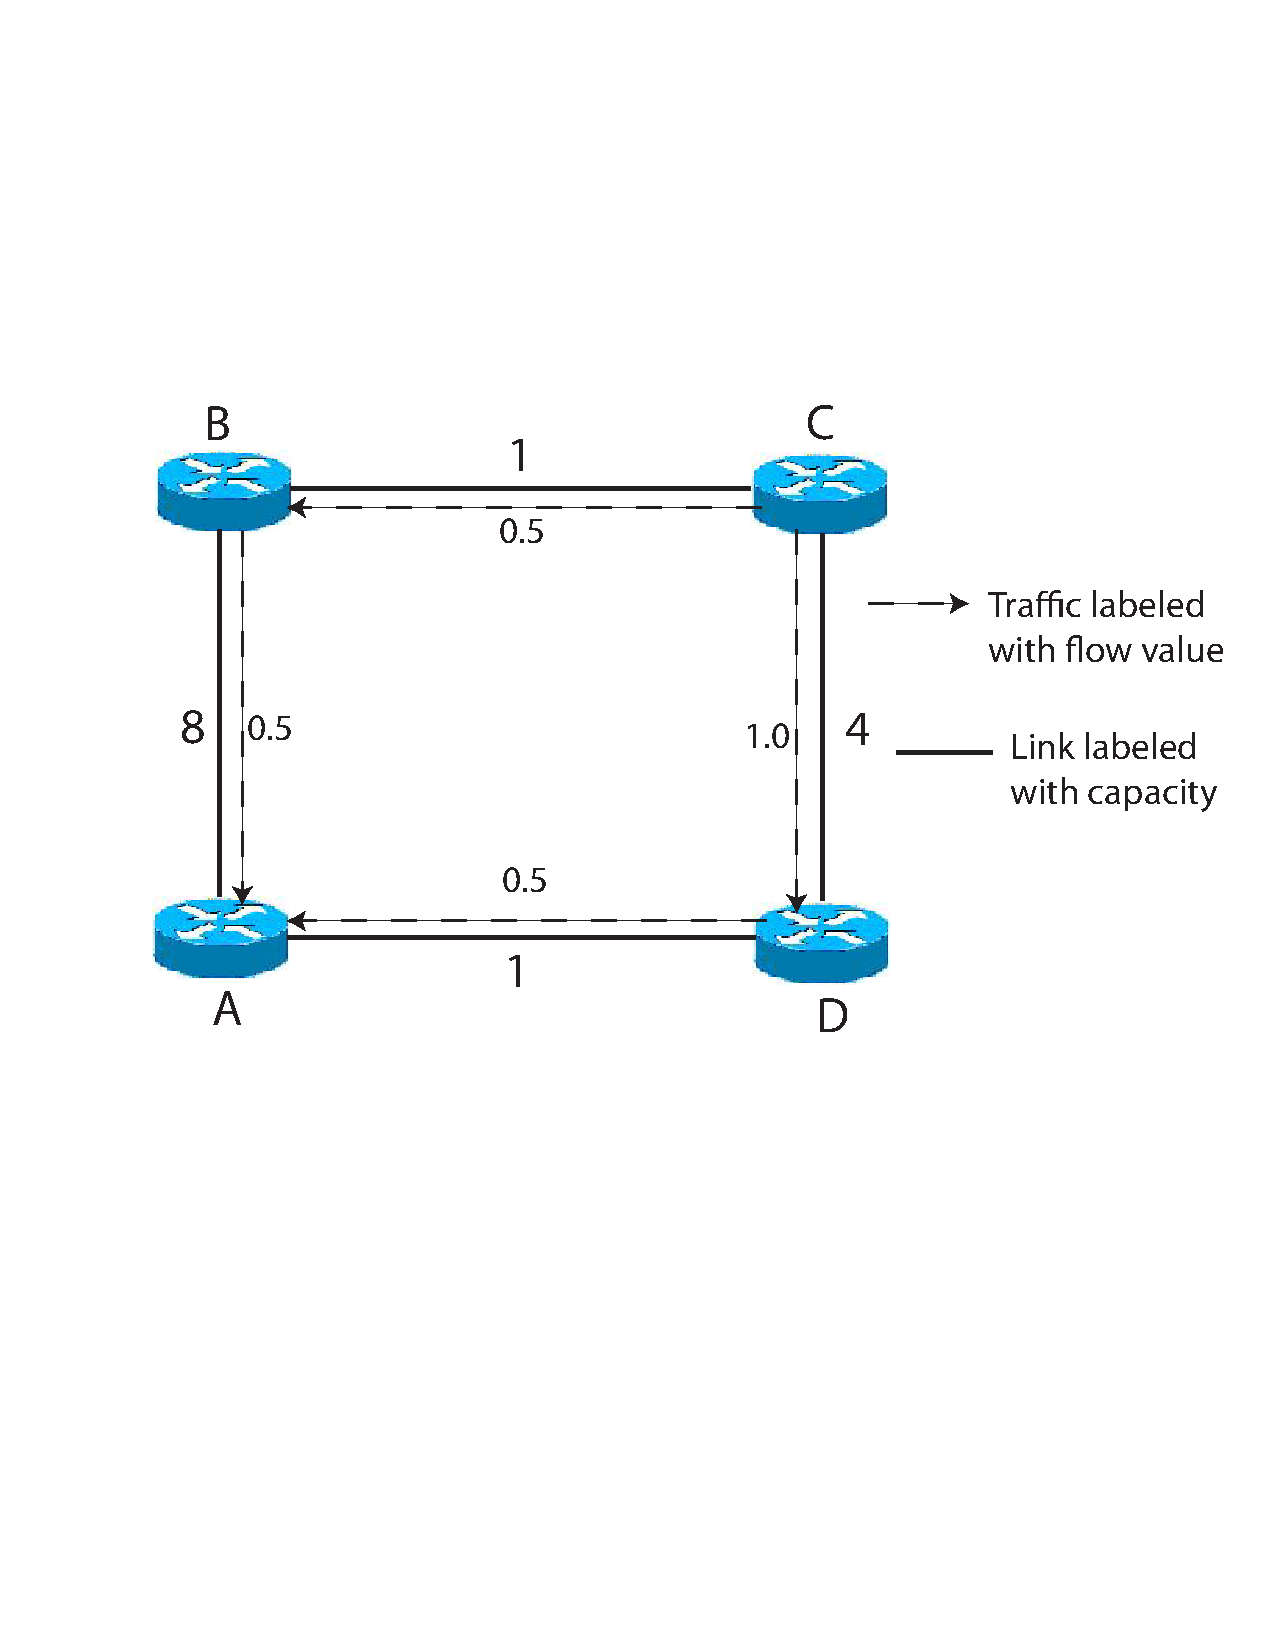
\includegraphics[width=2in]{NetworkExample}
\vspace{-1in}
\caption{A Simple \ncp\ Example}
\label{fig:NetworkExample}
\end{wrapfigure}
}

%On the other hand, NCDNs can shape the traffic demand matrix by using a judicious placement and redirection strategy. Suppose that there is some space left in the content server's cache at node $B$ to accommodate an additional copy of the demanded object. By creating an additional copy of the object at $B$, the traffic demand of $A$ can be satisfied from $B$ and the demand of $D$ from $C$ achieving the an MLU of $0.125$. In this case, judicious content placement decreased the MLU by a factor of $4$. Even more interestingly, this best MLU can be achieved using a simple routing scheme like InverseCap while also improving user-perceived latency (assuming that the latency of link $BA$ is lower than that of the two-hop paths from $C$ to $A$).

The prospect of  jointly optimizing placement, routing, and redirection raises several natural questions. How much additional benefit does such joint optimization offer compared to treating CDN and ISP concerns independently as practiced today? Is the added complexity of joint optimization strategies worth the benefit? Which of the three---placement, routing, and redirection---is the most critical to reducing network cost and user-perceived latency? How sensitive are these findings to characteristics of the content workload (e.g., video vs. download traffic)?

%Although this is clearly a ``toy'' example, it illustrates the sophisticated interaction between content placement and traffic engineering and potential opportunities for \ncp s to both reduce cost and simplify traffic engineering by doing it in a content-aware manner.

%NetworkExample
%
%\begin{figure}
%\centerline{\includegraphics[height=1.2in]{ncdnpaper/ncdn-example}}\vspace*{-0.1in}
%\caption{A simple \ncp\ example}
%\vspace*{-0.2in}
%\label{fig:NetworkExample}
%\end{figure}

%\begin{figure}
%\vspace*{-0.65in}
%\centerline{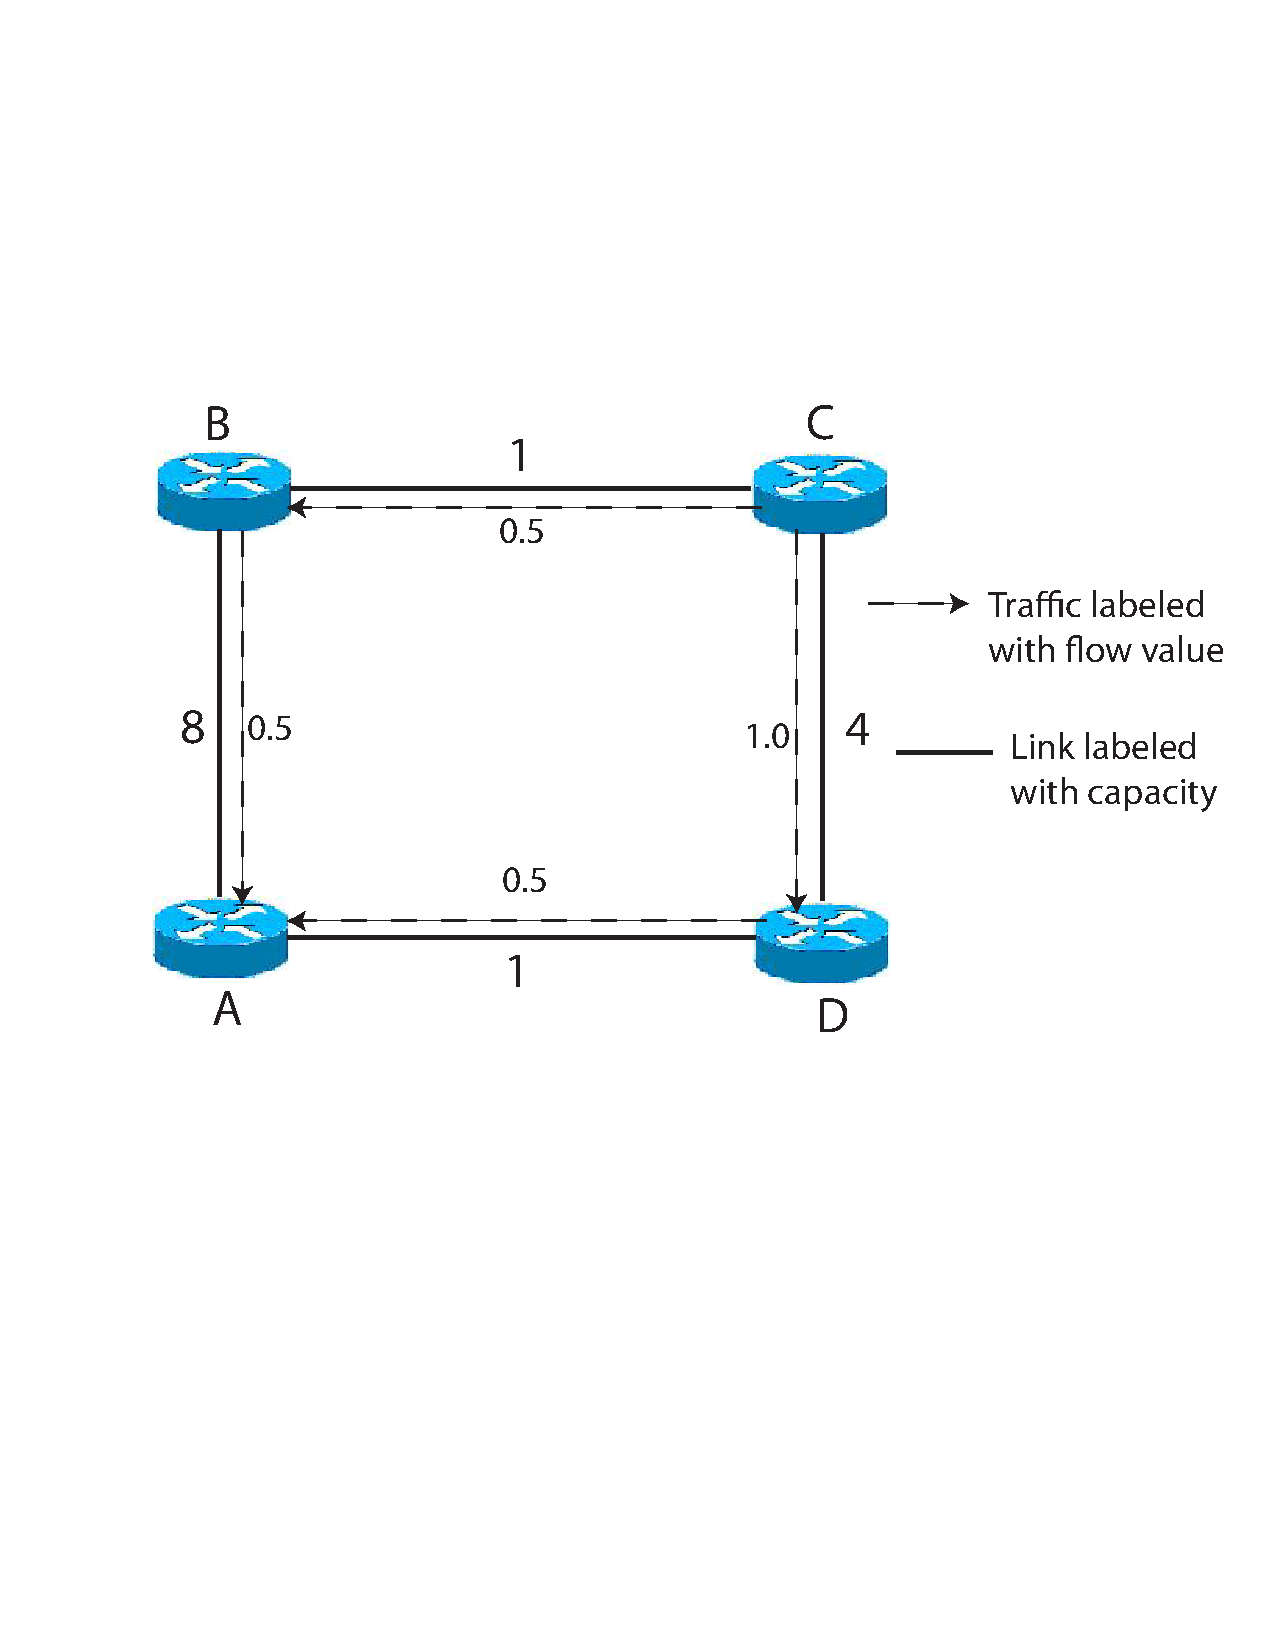
\includegraphics[height=3in]{NetworkExample}}
%\vspace*{-1.25in}
%\caption{A Simple \ncp\ Example}
%%\vspace*{-0.18in}
%\label{fig:NetworkExample}
%\end{figure}

%\section{Background}
%\label{sec:background}
%{\bf Network Model.} We model an NCDN as a graph where the nodes represent PoP's and the edges represent  backbone links that are provisioned between the respective PoPs (See Figure~\ref{fig:NCDNArch}). Each link has an associated capacity that represents the rate at which data can be transferred across that link. We assume that the content servers of the NCDN are deployed at every PoP with a specified amount of storage available at each node. The available storage is used for caching content. 

%A measure of how much storage is present in the network relative to the total content size is {\em replication factor}. Replication factor is the  ratio of the total storage available across all nodes in the network to the average unique content bytes accessed across the network per day. For instance, a replication factor of $k$ would mean that there is enough storage in the network to store (on average) $k$ copies of each unique content byte accessed per day.

%There are two types of costs involved in provisioning an NCDN: network cost for provisioning high-capacity links and cost for provisioning storage at each PoP. The network and storage costs typically have an inverse relationship. Increasing storage increases the ability to cache content closer to its demand, that in turn results in lesser traffic on the links. We explore this relationship in greater detail to help an NCDN determine the replication factor to needed to achieve its target network cost.

%{\bf Content Distribution Schemes.}  Content distribution has two key components: content placement and request redirection. Each of these components can be performed in multiple ways with differing levels of complexity. Content placement decides which objects needs to be cached at which node, potentially in a replicated fashion. Note that content placement can decide not to place an (unpopular) object in any of the nodes and instead serve it from origin. We distinguish two classes of content placement schemes. A {\em static} scheme for placement decides on a placement periodically (say, once a day) but does not alter its placement in between. In contrast, a {\em dynamic} scheme can continually alter the placement of objects after serving each request.  A simple example of dynamic placement is Least-Recently-Used (LRU) where each node serves the requested object. If the requested object is not in cache, it is added to the cache. If the cache is full, objects are evicted in the LRU order to make space for the new object. \tbd{Ramesh: Need to say something about request redirection here.}

%{\bf Intra-domain Routing Protocols.} We study traffic engineering under different intra-domain routing protocols. The most flexible but also the most complex is the MPLS protocol that allows traffic between nodes to be split arbitrarily and be routed on an arbitrary set of paths. Less flexible but less complex is OSPF where each link is associated with weights and traffic between two nodes is routed on the shortest path between the nodes using the weights as the lengths of the links. The least flexible but also the simplest is a special case of OSPF where the weight of each link is simply the inverse of its capacity (InvCap). InvCap routing is commonly used  due to its simplicity and is in fact the default setting in Cisco routers.

%{\bf Content-aware Traffic Engineering.} 
%The goal of traffic engineering is to route traffic demands on the network with the smallest MLU, i.e., minimize the utilization of the most congested link in the network. This ensures that network resources are utilized in an optimal fashion and leaves the maximum headroom for a traffic surge in the network. Our central thesis is that one can place the content in the network in a manner that ``shapes'' the traffic demands so that they are routable with significantly smaller MLU. Further, the smaller MLUs are obtainable even with the simplest routing protocols such as InvCap, rather than having to implement more complex OSPF schemes or the  MPLS protocol.  

\eat {
\begin{figure}
\centerline{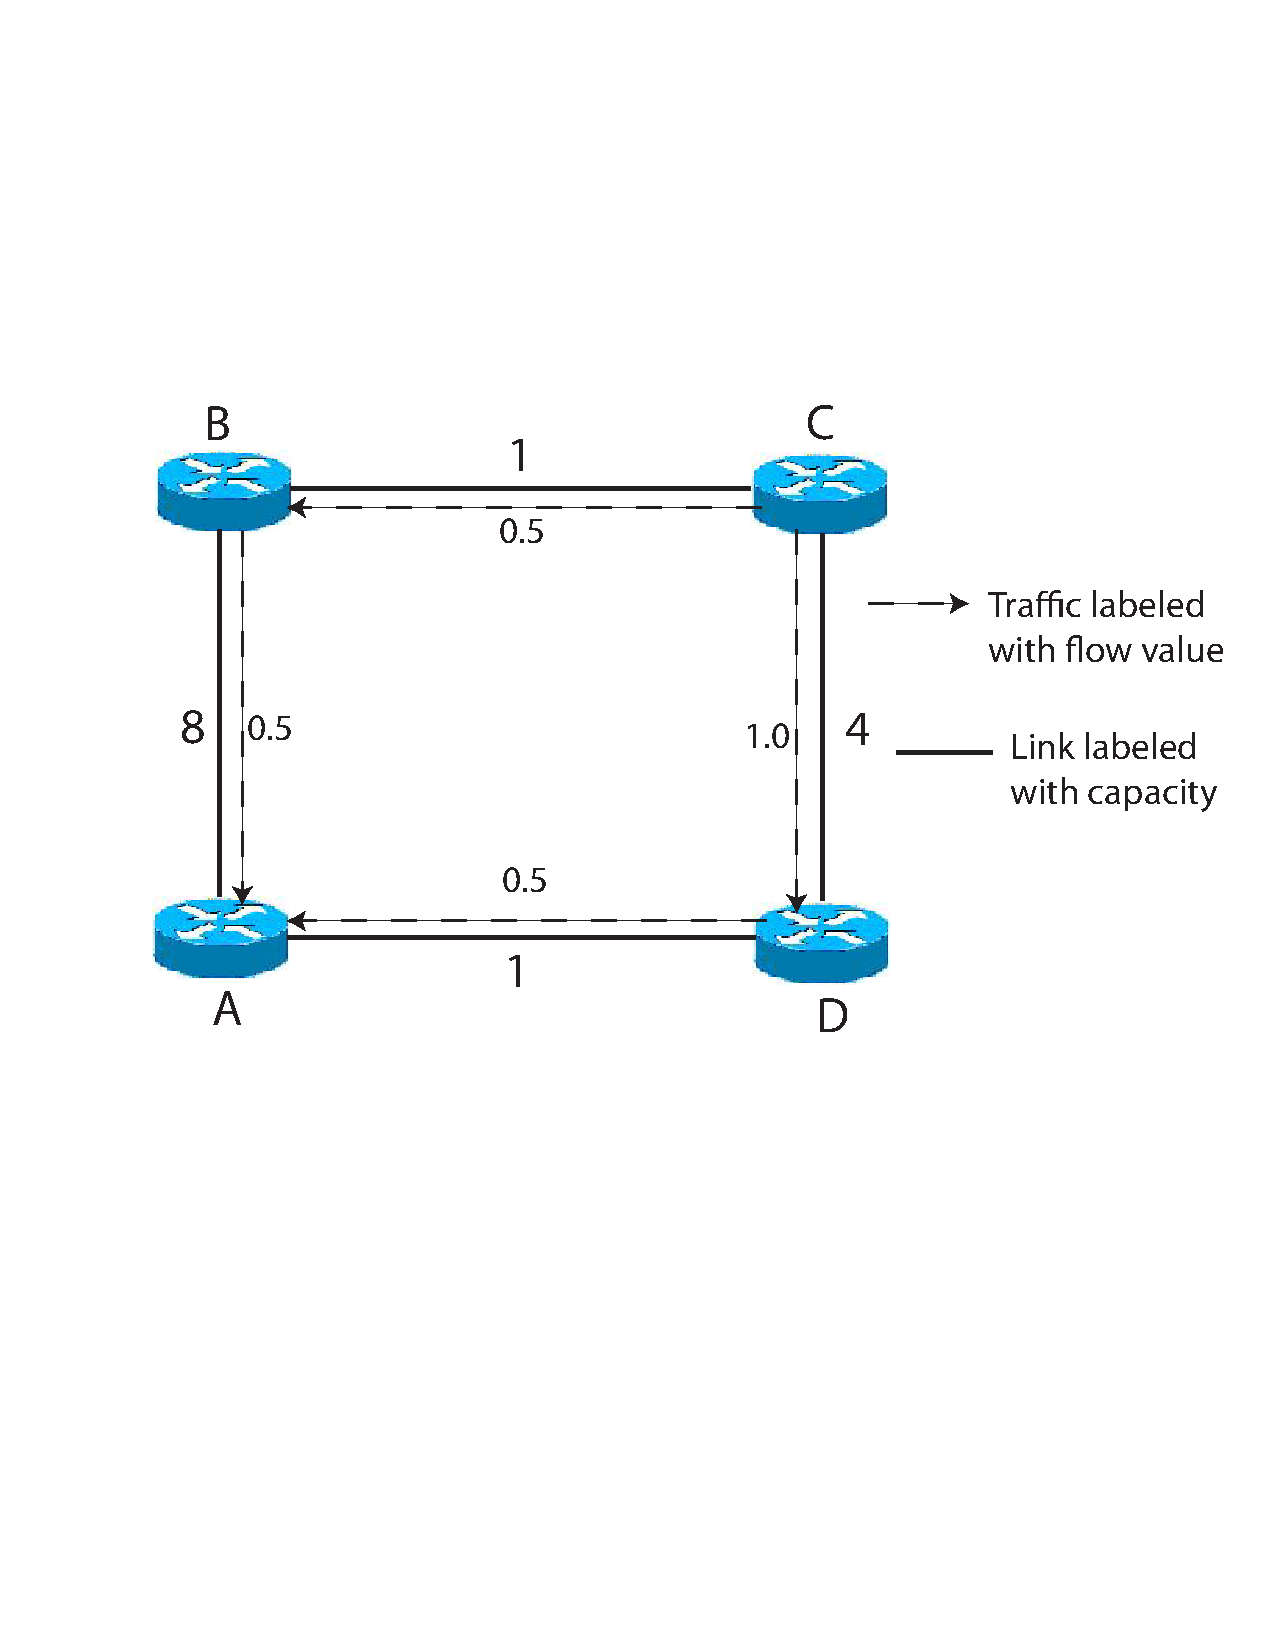
\includegraphics[height=4in]{NetworkExample}}
\vspace*{-1.5in}
\caption{A Simple Network Example}
\label{fig:NetworkExample}
\end{figure}
}

%To illustrate the central thesis with a simple suggestive example, assume that in the network of Figure~\ref{fig:NetworkExample} node $C$ has an object in its cache that is requested by end-users at nodes $A$ and $D$. Suppose that one unit of traffic needs to be routed from $C$ to $A$ and $0.5$ units  from $C$ to $D$ to satisfy the demand for that object. The routing that achieves the minimum MLU of $0.5$ to serve the demanded object is shown in the figure. Further note that the paths that achieve MLU of 0.5 are not routable with the InvCap protocol, since InvCap would route all the traffic demand from $C$ to $A$ via $B$, causing an MLU of 1. In traditional traffic engineering, the traffic demand matrix to be routed cannot be changed. But, with the additional power of content distribution, we can ``shape'' the traffic demand matrix by content replication and placement. Suppose that there is some space left in the content server's cache at node $B$ to accommodate an additional copy of the demanded object. By creating an additional copy of the object at $B$, the traffic demand of $A$ can be satisfied from $B$ and the demand of $D$ from $C$ achieving the an MLU of $0.125$. In this case, judicious content replication decreased the MLU by a factor of $4$. Further, note that the best MLU can be achieved using the much simpler InvCap routing protocol. While this is clearly a ``toy'' example, it is an illustration of the sophisticated interaction between content placement and traffic engineering that we exploit using algorithms that jointly perform both functions.


%\noindent\textbf{Video traffic growth is increasing backbone traffic for ISPs}

%The problem of network cost optimization through traffic engineering (TE)  in Internet Service Provider (ISP) networks has risen in importance due to current and projected growth of video traffic  in the Internet  \cite{nielsen-video-growth,cisco-videogrowth}. In order to cope with this surge in traffic, ISPs are going to need effective strategies to minimize the increase on backbone traffic or else incur expensive link capacity upgrades.
% Top Internet video websites, including Youtube, Hulu and Netflix have witnessed  at staggering 45\% increase in average time spent by users  in January 2011 over the past year \cite{nielsen-video-growth}.According to a well-publicized Cisco report \cite{cisco-videogrowth}, ``Internet video is now (year 2010) 40 percent of consumer Internet traffic, and will reach 61 percent by the end of 2015" and ``the sum of all forms of video (TV, video on demand, Internet, and P2P) will continue to be approximately 90 percent of global consumer traffic by 2015". The global IP traffic is expected to increase from 20 exabytes per month in 2010 to 81 exabytes per month in 2015, of which 33 exabytes of increase in traffic is expected to be contributed by Internet video alone (excluding other forms of video).  
 

%\noindent\textbf{ISPs turning into Network CDNs }

%An ongoing trend among many ISPs worldwide is to offer content delivery services through their network \cite{telco-cdn-list, att-cdn, verizon-cdn, level3-cdn}. We call these ISPs Network-CDNs  \footnote[1]{Network-CDN is also known by the names of Telco-CDN/Carrier-CDN.}.  An extra dimension of control which a Network-CDN enjoys over a traditional ISP is that it can decide the \emph{content placement} in the network for content served through its CDN service. A content placement strategy determines which locations to store  a content in the network and to which location should a user's request be redirected. An effective content placement strategy can significantly reduce the network cost for a Network-CDN. This is because content popularity distribution is known to follow power-law distributions, therefore replicating popular content at many locations significantly reduces the aggregate traffic in the network. 

%\noindent\textbf{Content placement determines backbone traffic.}

%An important determinant of backbone traffic in the Internet is the content placement strategy being used. A content placement strategy determines the location/s where content is placed in a network and the location where a user's request is redirected to. An example of a content placement strategy is distributed caching, where each user's request is first sent to the cache closest to the user. If a cache miss occurs at the closest cache, the content is fetched from the nearest cache where it is available and served to the user. 

%\noindent\textbf{Traffic Engineering in Network CDNs: content placement + routing}

%\subsection{Traffic Engineering Strategies}
%\label{sec:tescheme}
%In this paper, we study the problem of network cost optimization or traffic engineering for a Network CDN. Moreover, we focus only on the traffic inside a Network-CDN due to its CDN service.  For the traffic from its CDN service, a Network-CDN can optimize its network cost through two mechanisms - content placement and routing.    


%A very simple TE scheme which a Network-CDN can adopt is following: (1) Use a static shortest path routing using OSPF where the link weights are set using inverse of link capacity. This specific weight setting is the default configuration in Cisco routers. We use the term InvCap to denote this routing strategy. (2) Use LRU Caching which is a simple content placement strategy.  First, because LRU Caching is already implemented in popular web servers such as Apache and Squid and second, it requires no prior knowledge of content demand.


%There are three ways in which a Network-CDN can improve upon the above TE scheme. 

%(1) Optimal routing + simple content placement (Opt R + LRU): Instead of using InvCap routing, a Network-CDN can use previously measured traffic matrices in order to compute an optimal routing based on those traffic matrices. This approach is identical to traffic engineering done by ISPs today. 
%(2) Optimal  content placement + simple routing (InvCap + Opt P): Instead of LRU Caching, it can pre-compute the content placement using previously measured traffic demands, and statically place content at computed locations.  Such an approach has been shown to yield improved network cost for VoD content. 
%(3) Optimal  content placement + optimal routing (Opt R + Opt P): It can jointly optimize both content placement and routing. There are more TE schemes which a Network-CDN can use,  for example,  using a combination of LRU Caching and Opt Placement.But, limit ourselves to these schemes in our discussion. 
%Note that all three above schemes are limited by the error in predicting the content popularity and/or traffic matrices. 
%A comparison of above schemes can give guidelines to Network-CDN on whether to optimize content placement or routing or both of them. If it is the case that optimizing content placement alone (InvCap + Opt P)  performs nearly the same as (Opt R + Opt P) and significantly better than (InvCap + LRU) and (Opt R + LRU), then a Network-CDN can optimize only the content placement and use a InvCap routing. But, if it is the case that both content placement and routing are equally important, i e., (Opt R + Opt P) significantly reduces network cost over (Opt R + LRU) and (Invcap + Opt P), then a Network-CDN should optimize both content placement and routing to optimize network cost.

%, depends on the importance of content placement relative to  routing

%\subsection{Effect of Storage on Network Cost}

%The performance of content placement schemes depends on storage available in the network. Since absolute value of storage may depend on the number and size of content being served, we use \emph{replication factor} as the storage metric. Replication factor is defined as the ratio of total storage at all nodes in the network to the the total size of content placed in the network. \footnote[2]{A CDN may choose not to place unpopular content in the network and leave it at the origin server.}.   

%On increasing the replication factor, the traffic on congested links and hence the network cost should reduce.  Let us consider the most congested link in the network as an example. As the number of copies of a content increases in the network, the fraction of requests for that content which need to use the most congested link  will monotonically reduce.  In the extreme case, if the content is present at all the nodes in the network, then the most congested link will receive no traffic due to requests for that content!

%Since the network cost depends on replication factor  and replication factor can vary from one Network-CDN to another, we need to evaluate all schemes for a wide range of replication factors.  The curve of network cost vs. replication factor thus obtained, can help a Network-CDN to determine the replication factor needed to achieve its target network cost.


%An answer to above questions favoring one over the other can give guidelines to Network-CDNs on where to invest their resources in order to manage the burgeoning Internet traffic.  Given that ISPs already use well-developed techniques for optimizing routing, if optimizing routing alone gives close to optimal network cost, it would suggest that Network-CDNs should continue to use existing traffic engineering techniques and optimizing content placement will further reduce  network cost minimally.  On the contrary, if optimizing content placement gives close to optimal network cost, then the focus of Network-CDNs should be on content placement optimization.


%%%%%%%%%%%%%%%%%%%%%% about content placement in CDNs %%%%%%%%%%%%%%%%%%%%%%%%%%%%

%Individually, both these mechanisms are used in Internet today. CDNs optimize content placement in order to load balance their servers and minimize the latency between users and servers. ISP optimize the routing in the network to minimize the network cost. But, there are three reasons why traffic engineering for a Network-CDN is different from content placement done by CDNs and routing as done by ISPs. 

%\noindent\textbf{Network cost minimizing content placement:}   First, a Network-CDN needs to find which content placement schemes  minimize the network cost.  

%To this end,  a Network-CDN cannot directly adopt  a content placement which minimizes a difference metric, such as the maximum load across servers at different locations or the average latency between users and servers.  For example, to minimize the maximum load on web servers,  a content placement strategy  can send send request to far off servers which are less loaded, thereby increase the aggregate traffic on links and increasing the network cost. Similarly, a placement strategy which minimizes latency without considering link capacity can increase network cost if a set of  highly popular content is placed at a node whose all outgoing links have low capacity. 


%This differentiates Network CDN traffic engineering from that of a traditional ISP which controls the routing, but not the content placement.   

%ISP today optimize the routing in the network to minimize the network cost. CDNs optimize content placement in order to load balance their servers and minimize the latency between users and servers. 



%Given the abundance of work on content placement techniques for content distribution networks, and traffic engineering for ISPs, a network CDN is unlikely to require a radical approach to either content placement or  routing. 

%But, there are three salient features of this problem which merit a re-evaluation of known techniques. 


%To resolve the posed question, we also need to know which content placement schemes minimize  network cost for content which are major contributors of Internet traffic. But the answer to this question is not well known. A recent study by Applegate et al \cite{Applegate04} analyzes this problem for a IPTV  service which provides on demand videos. A similar analysis for video from another major sources, e. g. Internet short-form and long-form video, is still an open question.


%\noindent\textbf{Relation between replication factor and network cost:}  Replication factor is defined as the ratio of total storage at all nodes in the network to the the total size of content placed in the network. \footnote[2]{A CDN may choose not to place unpopular content in the network and leave it at the origin server.}.   

%On increasing the replication factor, the traffic on congested links and hence the network cost should reduce.  Let us consider the most congested link in the network as an example. As the number of copies of a content increases in the network, the fraction of requests for that content which need to use the most congested link  will monotonically reduce.  In the extreme case, if the content is present at all the nodes in the network, then the most congested link will receive no traffic due to requests for that content!

%Since the network cost depends on replication factor  and replication factor can vary from one Network-CDN to another, we need to evaluate content placement schemes for a wide range of replication factors.  The curve of network cost vs. replication factor thus obtained, can help a Network-CDN to determine the replication factor needed to achieve its target network cost.

%\noindent\textbf{Importance of content placement relative to routing:} Since a Network-CDN can minimize the network cost through content placement as well as routing, it is intuitive to ask the following question: \emph{Is optimizing content placement or optimizing routing more important to reduce the network cost for a Network-CDN?}






%Optimizing routing reduces network cost by exploiting the \emph{path diversity} in the network. 

%An intelligent content placement strategy helps reduce network cost by maximizing the \emph{location diversity} of content, i.e. the number of locations at which content is available.  Routing optimization is constrained by the path diversity available in the network.  Analogously, content placement is constrained by the storage at nodes. 

%A constraint on increasing the location diversity  is the storage available at each location. Intelligent content placement can make the best use of available storage, by replicating content based on its popularity. For example, a highly popular content gets replicated at many more locations than an unpopular content, which reduces backbone traffic significantly in spite of storage constraints. Intelligent content placement can also exploit the skew in content popularity at different locations; the content popularity may be highly skewed for some content across different locations. By placing content at more popular locations, content placement can further optimize network cost. 


%As  location diversity of content increases in the network, a user is able to get the content by crossing lesser number of links on average. This reduces the aggregate backbone traffic generated due to content accesses.  



%An intelligent content placement strategy helps reduce backbone traffic by maximizing the locality of content accesses.  The lesser number of links each users' request traverses, the lesser is the aggregate backbone traffic. A constraint which any content placement strategy faces is the storage available at each location. By choosing to replicate popular content at more locations helps maximize locality for a high fraction of requests, in spite of storage constraints.  All content is not equally popular at all locations. Therefore, intelligent content placement can further maximize locality by placing content at locations where its most popular.










%By choosing to replicate popular content at more locations helps maximize location diversity for a high fraction of requests, in spite of storage constraints.  All content is not equally popular at all locations. Therefore, intelligent content placement can further maximize locality by placing content at locations where its most popular.


 
%We assume that a Telco CDN can measure the PoP level demand for each content in order to decide its placement as well as routing in the network. This serves a similar purpose as measuring traffic matrices by an ISP for traffic engineering \cite{ZhangTMEst1,ZhangTMEst2}.


%To minimize the network cost for this traffic,  a Network-CDN can make decisions about content placement and well as routing. 

%A Network-CDN controls content placement for the content it is distributing through its CDN service. 

%In our discussion, we focus only on the traffic due to content distributed through the CDN service of a Network-CDN.  A Network-CDN controls the content placement for the content distributed through its CDN service, and since it is the network owner, it also controls the 

%A Network-CDN has the advantage over a traditional ISP in that it controls content placement as well as routing and therefore can possibly better optimize its network cost. A Network-CDN can have traffic due to content for which it cannot control content placement but we do not consider that as a part of our discussion.

% to increase their portfolio of services. We call these ISPs Network-CDNs. We believe an added incentive for Network-CDNs is that they can control content placement in their network which enables them to reduce their network cost. Moreover, Network-CDNs also control routing in their network like traditional ISPs. A Network CDN can have traffic due to content for which it cannot control content placement but we do not consider that as a part of our discussion. 



%Collectively, content placement and routing both can be optimized for traffic engineering in a Network-CDN since both of those determine the network cost. Optimizing routing in a traditional ISP exploits the \emph{path diversity} available in an ISP network. Similarly, optimizing content placement in a Network CDN, exploits the \emph{location diversity} available in a Network-CDN. 






%\noindent\textbf{case for network-cdns}

%We analyze the above question in the context of Network-CDNs. An ISP which offers content distribution services through its network is called a Network-CDN.  Major ISPs today including AT\&T, Verizon, Level-3  offer content distribution services, and hence can be called Network-CDNs.A Network-CDN has the advantage over a traditional ISP in that it controls content placement as well as routing and therefore can possibly better optimize its network cost. 

% While their primary purpose is to 
% to increase their portfolio of services. We call these ISPs Network-CDNs. We believe an added incentive for Network-CDNs is that they can control content placement in their network which enables them to reduce their network cost. Moreover, Network-CDNs also control routing in their network like traditional ISPs. A Network CDN can have traffic due to content for which it cannot control content placement but we do not consider that as a part of our discussion. 

% leverage the advantage of content placement in reducing network cost and for added revenue, . We call such ISPs as  Network-CDNs.  To provide CDN services, a Network-CDN has the storage and server infrastructure in its network.


%\noindent\textbf{Network-CDNs are at an advantage in optimizing network cost since they can optimize content placement in addition to routing}

%A Network-CDN�differs from a traditional ISP in that it controls both the \emph{content placement} and routing in the network while a non-CDN ISP only controls routing. A Network CDN can have traffic due to content for which it cannot control content placement but we do not consider that as a part of our discussion. 


%\noindent\textbf{TE in Network-CDN = content placement + routing}

%Collectively, content placement and routing both can be optimized for traffic engineering in a Network-CDN since both of those determine the network cost. Optimizing routing in a traditional ISP exploits the \emph{path diversity} available in an ISP network. Similarly, optimizing content placement in a Network CDN, exploits the \emph{location diversity} available in a Network-CDN. 



%This leads us to the central question we seek to answer: 

%\begin{center}
%\emph{Is optimizing content placement or optimizing routing more important to reduce the network cost for Network-CDN ?}
%\end{center}


%\noindent\textbf{Implications}








%We call the combination of content placement scheme and routing scheme being used by a Network-CDN as a traffic engineering scheme.


%To choose the best traffic engineering scheme for a Network-CDN, we need to consider the set of content placement strategies and routing strategies.


%Network CDN traffic engineering consists of optimizing content placement and optimizing routing in the network.

%Traffic engineering for an ISP  (non-CDN)  translates to optimizing the routing in the network. For a Network-CDN, routing decision as well \emph{content placement} decisions affect the network cost. Hence, 
%The goal of traffic engineering problem is to reduce a network cost function. The network cost function depends on the link utilization. 

%The traffic engineering (TE) problem for a Network-CDN is to determine routing in network as well as content placement and redirection strategy so as to optimize a network cost function.   The network cost we use is maximum link utilization (MLU), a commonly used network cost function. 



%%%%%%%%%%%%%%%CLASSIFICATION OF STRATEGIES
%
%\subsection{A Classification Of Strategies}
%
%We now describe different classes of traffic engineering schemes which a Network CDN can adopt in its network. We first describe content placement strategies followed by routing strategies.
%
%\subsubsection{Content Placement Strategies}
%
%%Broadly, there are two ways to solve the placement part of this problem. One approach is to precompute a placement based on previously measured demands and second approach is to use a caching strategy to determine content placement. A combination of static and dynamic placement strategies can also be used. 
%
%We classify placement strategies into three classes: static placement, which assigns a set of fixed locations for each content, dynamic placement or caching,  and hybrid placement, a combination of static and dynamic placement. We describe each of these strategies below.
%
%\noindent\textbf{Dynamic Placement:}
% Dynamic placement or caching maintains a cache, for example an LRU cache, at each PoP. When a user connected through a PoP asks for a content which is not present at the PoP, the content is delivered from another PoP in the network or the origin, and cached at this PoP. Hence, location of content is continuously changing depending on the access pattern in the network. A combination of static and dynamic placement strategies can also be used. 
%
%\noindent\textbf{Static Placement:}
%A static placement assigns a set of fixed locations for each content. Locations for each content do not change until the placement is recomputed again after some interval.
%
%\noindent\textbf{demand unaware static placement}
%
%Some static placement strategies require measuring the content popularity  while others don't. An example of the latter strategy is as follows - place the same number of copies of each content in the network subject to storage constraints; locations for each content are chosen randomly. A simple redirection scheme can be used with this strategy - send a user to the nearest copy of the content based on latency. It is expected that such a scheme will perform poorly because not all content have same popularity and content popularity is not the same at all locations.
%For example, a highly popular content should be stored at more locations than an unpopular content when available storage is a constraint. This is because the reduction in backbone traffic due to a content being accessed from a nearby location by users is much more for a highly popular content than for unpopular content. Therefore it seems useful for a Network-CDN to invest in infrastructure to measure the content popularity.
%
%
%\noindent\textbf{demand aware static placement - heuristic and optimal}
%
%Static placement schemes which use the content popularity measurement can calculate an optimal placement using this information.  The only approach that we are aware of for calculating an optimal placement is through solving a MIP similar to that presented in Section \ref{sec:optmip}. Applegate et al. \cite{Applegate2010} show that optimizing content placement for a network model similar to one we are considering is tractable for large content libraries but still their solution takes two hours to complete even with state of the art optimization techniques.  Therefore, heuristics for static content placement  which trade optimality for faster computation represent another possible class of strategies. We present one such heuristic in Section \ref{sec:heuristic}.
%
%
%
%
%\noindent\textbf{Hybrid (Dynamic + Static) Placement:} A combination of static and dynamic placement schemes can also be used. Such a scheme entails dedicating a fraction of the storage at some or all of the PoP/s to act as a cache for content while filling up the remaining storage using a static placement strategy. Adding dynamic placement can potentially improve a purely static placement scheme. For example,  if a new content is added whose popularity is yet unknown or the popularity for a previous unpopular content suddenly increases. In these cases dynamically caching the content based on demand is likely to improve performance.
%
%\noindent\textbf{Redirection Strategies:}
%
%
%
%\subsubsection{Routing Strategies}
%
%\noindent\textbf{offline optimal and simple static shortest path}
%
%We present two routing strategies for a Network CDN: Offline Optimal and Static Shortest Path Routing. 
%Offline Optimal is inspired by current traffic engineering practice among ISPs. 
%ISPs today do ``offline" traffic engineering, using  either OSPF \cite{ospf-cite} or MPLS \cite{mpls-cite}. 
%The word offline comes from the fact that routing is computed on paper using previously measured traffic matrices and then implemented in the network. 
%Analogous to offline traffic engineering, a Network CDN, can compute routing using previously measured traffic matrices and then implement in the network. 




%\begin{enumerate}
%\item
%Simple Routing + Simple Placement:   Two such strategies are (1) (InvCap Routing + Random Placement + InvCap Flow Splits)  (2)  (InvCap Routing + Random Placment + InvLatency Flow Splits)
%
%\item
%Optimal Routing + Simple Placement:  Two such strategies are (3) (Optimal Routing + Random Placement + InvCap Flow Splits)  (4)  (Optimal Routing + Random Placment + InvLatency Flow Splits). This can be calculated  using the linear program described in Section \ref{sec:optrouting}
%
%\item
%Simple Routing + Optimal Placement: We propose the following strategy: (5) (InvCap Routing + Optimal (Placement + Flow Splits). This can be calculated  using the linear program described in Section \ref{sec:optplacement}
%
%\item
%Optimal Routing +Placement :  This is the joint optimal routing and placement strategy (6) which can be calculated using the  MIP in Section \ref{sec:optmip}.
%\end{enumerate}
%
%To understand the benefits of optimizing flow splits, we evaluate the following scheme (7) (InvCap Routing + Random Placement + Optimal Flow Splits)
%
%There are three things that an \ncp\ needs to consider - (1) content placement , (2) flow splits  and (3) routing in the network. 
%
%We compare follwing schemes: 
%
%(1) Optimizing content placement, flow splits and routing: standard for comparison. 
%
%(2) Optimizing content placement, optimal flow splits but simple static routing: as good as optimal. shows that we can stop optimizing routing if we are optimizing other two.
%
%(3) Optimizing content placement keeping flow splits and routing simple: change the placement of the content if popularity changes but keep a simple static routing and even the flow splits algorithm simple. (what about the cost of switching from one placement to another ?)
%
%(4) Optimizing flow splits keeping placement and routing simple: compute flow splits optimally in the network if the content popularity changes. change content placement using a simple algorithm and keep a simple static routing. 
%
%(4) Optimizing routing keeping content placement and flow splits simple: just optimize routing but keep other things simple
%
%(5) Keeping content placement, flow splits and routing simple: keep everything simple
%
%(6) Using LRU cache replacement for placement, with simple flow splits and simple routing: use a cache replacement strategy for placement, a simple placement strategy with a simple routing
%
%(7) Using LRU cache replacement for placement, with simple flow splits and optimal routing: same as prev scheme but optimize routing as well : how do you  optimize routing




%\subsection{Time varying traffic demands}
%A constraint with time varying demands is that content placement cannot be changed very frequently. Therefore, we assume that placement changes at a slower time scale than routing.
